\section{PCA Model Order Reduction for Bound Computation}

%Some words on PCA, learn of 2 Matrix full-dim to reduced-dim and back.
%Then, how we use it (pictures and text).

\begin{figure*}[h!]
    \centering
    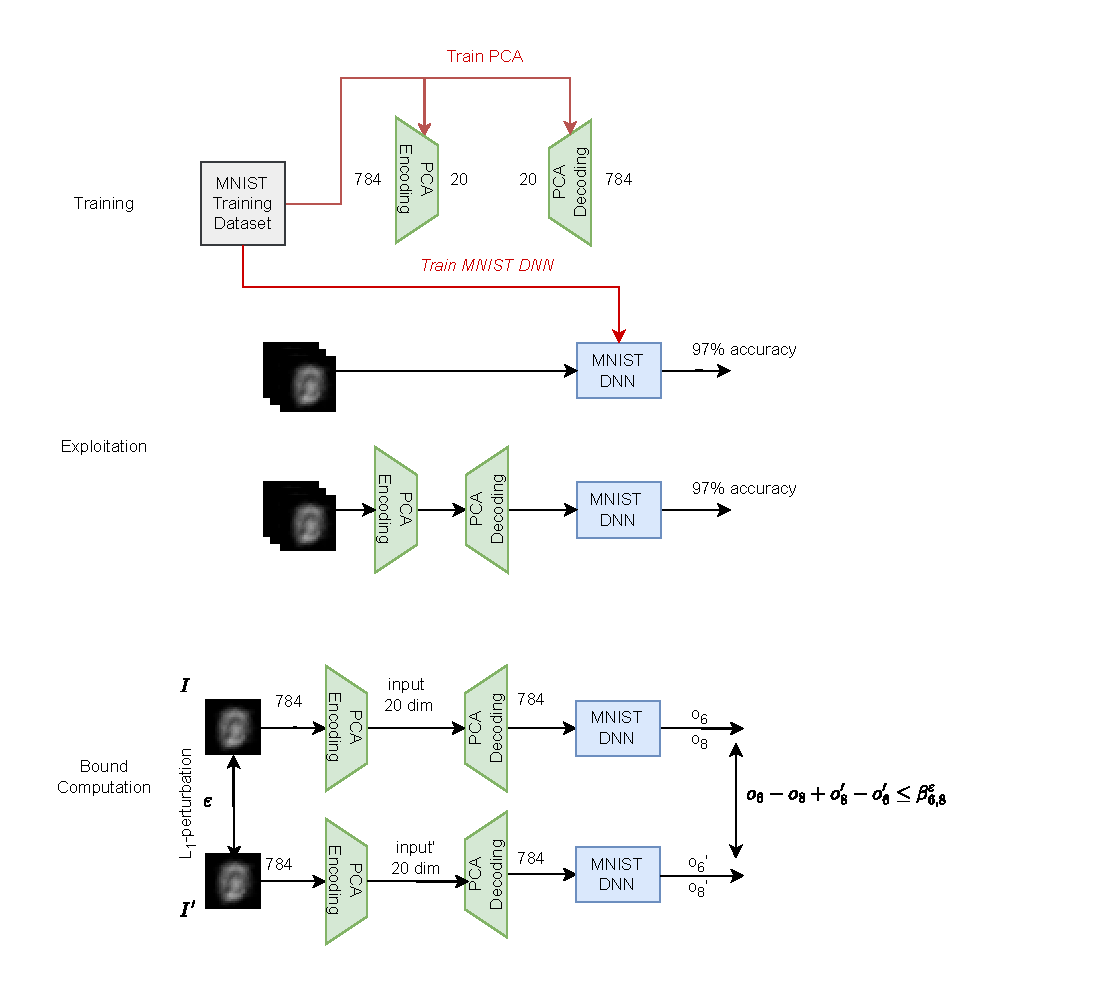
\includegraphics[scale=0.9]{MNIST.pdf} \hspace{1.5cm}
    \caption{Training, exploitation, and bound computation on the MNIST dataset.}
    \label{fig.MNIST}
\end{figure*}	

\begin{figure*}[h!]
    \centering
    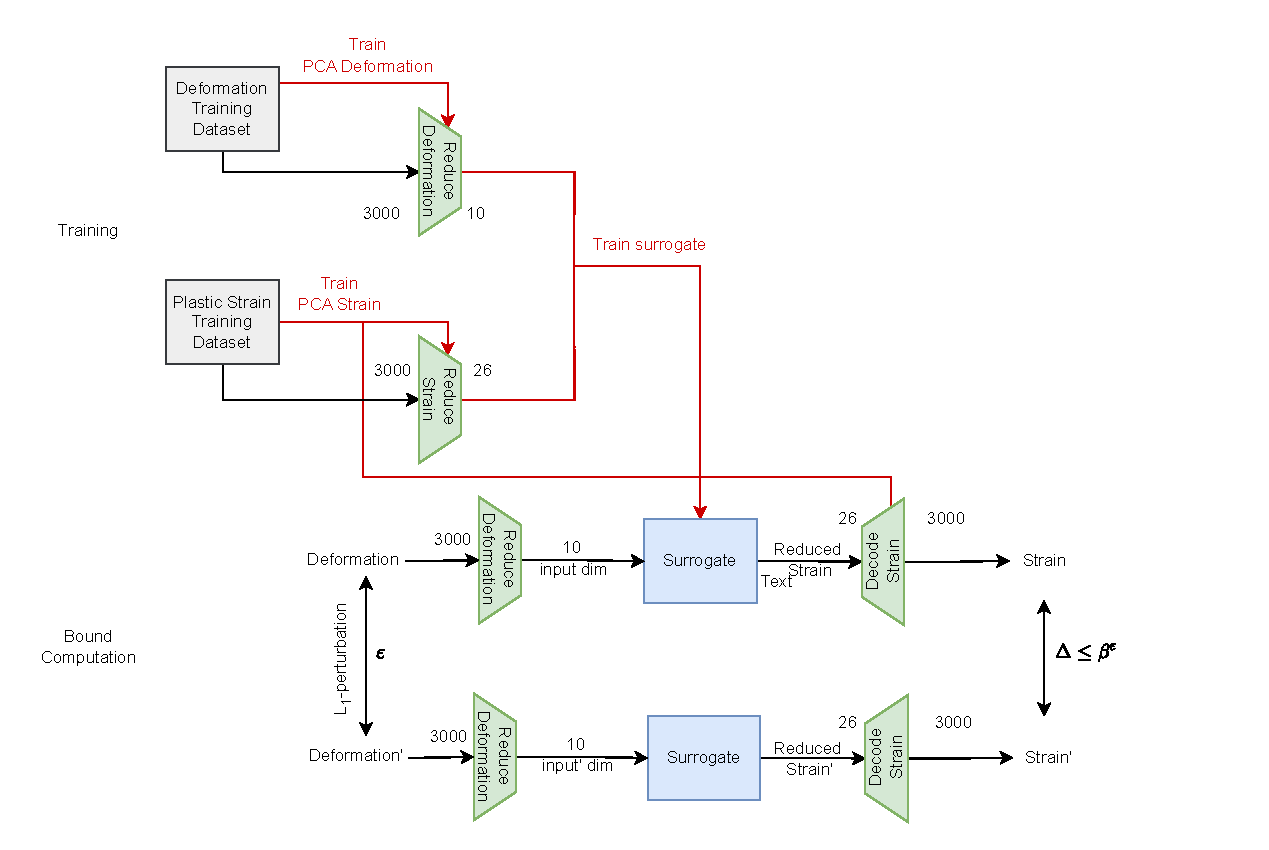
\includegraphics[scale=0.9]{PIPE.pdf} \hspace{1.5cm}
    \caption{Training and bound computation on the pipe use case. 
    Note that two PCAs are used, one for the input space (deformation) and another for the output space (plastic strain). The exploitation and bound computation must then use a pipeline that: (1) reduces the deformation; (2) obtains a reduced strain with the surrogate, and (3) decodes the reduced strain from the reduced to the full dimension.}
    \label{fig.PIPE}
\end{figure*}	


PCA (Chinesta et al. 2017) is a linear technique to reduce the dimension of a dataset while keeping its main information.
From a dataset, the eigenvectors are computed, defining the most important linear components of this dataset.
Projecting over the first few main eigenvectors is a powerful model order reduction technique ({\em encoding} / {\em reducing from the full dimension}). 
It is easy to go from the reduced dimension back to the full dimension
by making the product between the reduced vector and the first few eigenvectors ({\em decoding}).

Figure~\ref{fig.MNIST} depicts the MNIST pipeline on reduced dimensions, computing:

\begin{enumerate}
\item the PCA encoding and decoding as well as the MNIST DNN from the MNIST Training DataSet ({\em Training}).
We choose to reduce the dimension from 784 to 20, using the first 20 eigen vectors from PCA, with a PCA encoder and a PCA decoder.

\item {\em In exploitation}, we check whether a test dataset has the same accuracy (class predicted matches the ground truth) 
going directly through the MNIST DNN rather than being encoded and decoded by the PCA decoding first.
The number of retained PCA dimensions (20) is selected to ensure that the MNIST DNN's classification accuracy on reconstructed images (i.e., after PCA encoding and decoding) remains the same $97$\% as the MNIST DNN used directly on the full-dimensional MNIST images.
It ensures no loss of accuracy.
%
\item {\em In Bound Computation}, we consider as input the 20 ($\times 2$: input and perturbed input') reduced PCA dimensions, from which all other variables are fixed.
However, we can define 784 $\times 2$ linear variables corresponding to the original image $I$ and its perturbation $I'$ before PCA encoding, as the constraints between these and the input are linear.
We fix the $L_1$-perturbation $\varepsilon$ on the image $I$ and its deformation $I'$, rather than on the inputs, as that is where it is meaningful.
Finally, the goal is to optimize the value of $o_6 -o_8+ o'_8 - o'_6$,  where $o_C$ is the output neuron of the DNN corresponding to class $C \in \{0,\ldots, 9\}$.
\end{enumerate}

%
%It was also used to obtain the PCA encoding and decoding, transforming the images into a reduced basis. The number of PCA dimensions was chosen such that the exploitation accuracy remains constant. That is, encoding into a PCA basis and decoding it results in the same accuracy, as illustrated in ``Exploitation''. 
%
%Last, for the ``bound computation'', we determine an $L_1$-perturbation $\varepsilon$. The search space for bound computation is 20-dimensional. However, the bound itself is computed on the full space. This is possible since PCA is a \emph{linear operation} based on the eigenvectors of the covariance matrix and its transpose for the PCA decoding (inverse).

\newpage


Figure~\ref{fig.PIPE} illustrates the pipeline used in the pipe strain case. 
Two different PCA reductions are used. The first one is on the deformation training dataset, 
and the second is on the plastic strain one.
%
The surrogate is then learned from the reduced deformation to the reduced plastic strain. 
%

To predict the plastic strain (which is not directly observable), we thus consider the deformation (which is directly observable), reduce it using the PCA reduction to obtain the reduced deformation, call the surrogate model, obtain the associated predicted reduced strain, and decode the reduced strain, obtaining the strain of the pipe in the full 3000 dimensions. Similarly to the MNIST case, we consider as input the 10 $\times 2$ dimensions of reduced deformation, but also consider 3000 $\times 2$ linear variables corresponding to the deformation and its perturbation, with linear constraints between them and the inputs (provided by the PCA encoder, which is given under the form of a matrix), and set the $L_1$ perturbation $\varepsilon$ over the deformation and its perturbation, where it is physically meaningful.
The surrogate outputs 26 output dimensions ($\times 2$) of reduced strain, but again, as we have the linear PCA decoder explicitly, we can define the optimization goal in terms of optimizing the difference over 10 specific points in the full geometry (where it is are physically relevant), rather than on the reduced strain space.

\newpage

